\ifx\wholebook\relax \else
\documentclass[b5paper]{ctexart}
\usepackage[nomarginpar
  %, margin=.5in
]{geometry}

\addtolength{\oddsidemargin}{-0.05in}
\addtolength{\evensidemargin}{-0.05in}
\addtolength{\textwidth}{0.1in}
\usepackage[cn]{../../../prelude}

\setcounter{page}{1}

\begin{document}

\title{队列}

\author{刘新宇
\thanks{{\bfseries 刘新宇 } \newline
  Email: liuxinyu95@gmail.com \newline}
  }

\maketitle
\fi

\markboth{队列}{基本算法}

\ifx\wholebook\relax
\chapter{队列}
\numberwithin{Exercise}{chapter}
\fi

\section{简介}
\label{introduction}

队列提供了先进先出(FIFO)的机制。可以用多种方法实现队列,例如单向、双向链表,循环缓冲区等,Okasaki给出了16种不同的实现方法\cite{okasaki-book}。队列需要满足下面的两条基本要求:

\begin{enumerate}
\item 可以在常数时间内向末尾添加元素;
\item 可以在常数时间内从头部获取或删除元素。
\end{enumerate}

可以用双向链表直观地实现队列。我们略去这个简单的实现,而关注如何用其它基本数据结构,如列表、数组实现队列。

\section{列表实现}
\index{队列!单向链表实现}

我们可以用常数时间在列表头部插入、删除元素。但为了先进先出,我们只能在头部执行一种操作,而在尾部执行另一种操作。我们需要$O(n)$时间遍历整个列表以到达尾部,其中$n$是列表长度。这样就无法达到性能要求。为了解决这个问题,可以一个变量记录尾部位置。并用一个额外的节点$S$简化空队列的处理,如图\ref{fig:empty-list}所示。

\lstset{frame = single}
\begin{lstlisting}[language = Bourbaki]
data Node<K> {
  Key key
  Node next
}

data Queue {
  Node head, tail
}
\end{lstlisting}

\begin{figure}[htbp]
  \centering
  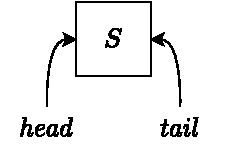
\includegraphics[scale=0.6]{img/empty-list}
  \caption{空队列,头、尾都指向$S$}
  \label{fig:empty-list}
\end{figure}

队列中最基本的两个操作是入队(Enqueue,或push、snoc、append、push back)和出队(Dequeue,或pop、pop front)。使用列表时,我们选择在头部加入元素、从尾部删除元素以简化实现。

\begin{algorithmic}[1]
\Function{Enqueue}{$Q, x$}
  \State $p \gets $ \Call{Node}{$x$}
  \State \Call{Next}{$p$} $\gets$ NIL
  \State \textproc{Next}(\Call{Tail}{$Q$}) $\gets p$
  \State \Call{Tail}{$Q$} $\gets p$
\EndFunction
\end{algorithmic}

队列至少有一个节点(空队列中有$S$节点),因此无需检查尾部是否为NIL。

\begin{algorithmic}[1]
\Function{Dequeue}{$Q$}
  \State $x \gets $ \Call{Head}{$Q$}
  \State \textproc{Next}(\Call{Head}{$Q$}) $\gets$ \Call{Next}{$x$}
  \If{$x = $ \Call{Tail}{$Q$}} \Comment{$Q$变为空}
    \State \Call{Tail}{$Q$} $\gets$ \Call{Head}{$Q$}
  \EndIf
  \State \Return \Call{Key}{$x$}
\EndFunction
\end{algorithmic}

$S$节点在所有其它节点的前面,\textproc{Head}实际返回$S$的下一个节点,如图\ref{fig:list-queue}所示。我们可以把这一实现扩展到并发环境。在头部和尾部各使用一把并发锁。$S$节点可以在队列空时避免死锁\cite{PODC96}、\cite{SutterDDJ}。

\begin{figure}[htbp]
  \centering
  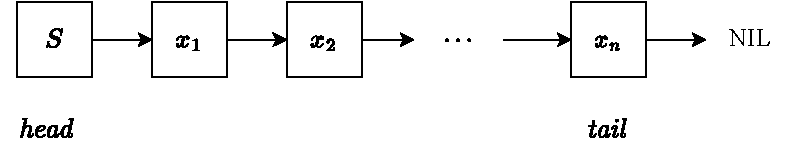
\includegraphics[scale=0.8]{img/slistq}
  \caption{带有$S$节点的列表}
  \label{fig:list-queue}
\end{figure}

\section{循环缓冲区}
\index{队列!循环缓冲区}

和列表相反,我们可以在常数时间将元素添加到数组末尾,但需要线性时间$O(n)$从头部删除。这是因为要将全部剩余元素依次向前移动。为了达到队列的性能要求,我们可以把数组的头尾连接起来,做成一个环,叫做循环缓冲区,如图如图\ref{fig:circular-buffer}、\ref{fig:circular-buffer-queue}所示。这样用数组的头部坐标head,队列长度count,和数组大小size,就可以完全表述队列。count等于0时队列为空,等于size时队列已满。我们还可以利用模运算简化入队、出队的实现。

\begin{figure}[htbp]
 \centering
 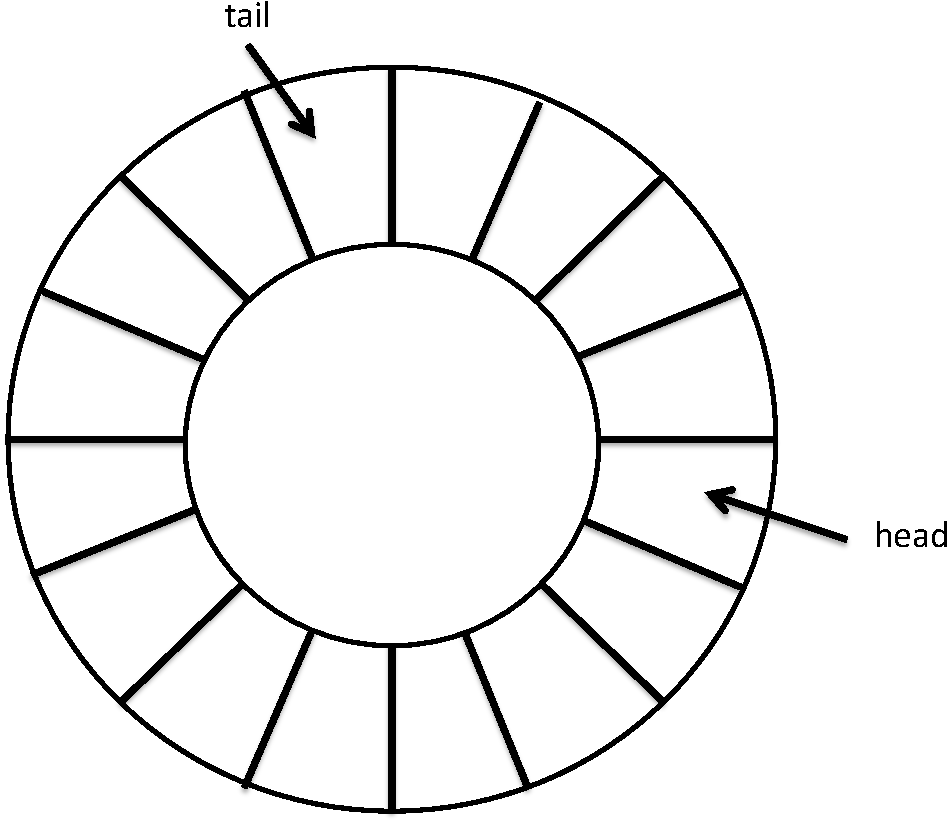
\includegraphics[scale=0.3]{img/ring-buffer}
 \caption{循环缓冲区}
 \label{fig:circular-buffer}
\end{figure}

\begin{figure}[htbp]
 \centering
 \subcaptionbox{连续加入多个元素。}{
 \begin{tikzpicture}[scale=0.8]
    \draw (0, 0) rectangle (1, 1) node (a0) [pos=.5] {a[0]}
          (1, 0) rectangle (2, 1) node [pos=.5] {a[1]}
          (2, 0) rectangle (3, 1) node [pos=.5] {...}
          (3, 0) rectangle (4, 1) node [pos=.5] (ai) {a[i]}
          (4, 0) rectangle (5, 1) node [pos=.5] {...}
          (5, 0) rectangle (6, 1) node (an) [pos=.5] {};
    \draw (0, 2) node (hd) {head}
          (3.5, 2) node (tl) {tail}
          (6, 2) node (bd) {边界};
    \draw[thick, ->] (hd) edge (a0)
                 (tl) edge (ai)
                 (bd) edge (an);
  \end{tikzpicture}}
 \subcaptionbox{从头部删除若干元素后,出现了空档。}{
  \begin{tikzpicture}[scale=0.8]
    \draw (0, 0) rectangle (1, 1)
          (1, 0) rectangle (2, 1) node [pos=.5] {...}
          (2, 0) rectangle (3, 1) node (aj) [pos=.5] {a[j]}
          (3, 0) rectangle (4, 1) node [pos=.5] {...}
          (4, 0) rectangle (5, 1) node (ai) [pos=.5] {a[i]}
          (5, 0) rectangle (6, 1) node [pos=.5] {...}
          (6, 0) rectangle (7, 1) node (an) [pos=.5] {};
    \draw (2, 2) node (hd) {head}
          (4.5, 2) node (tl) {tail}
          (7, 2) node (bd) {边界};
    \draw[thick, ->] (hd) edge (aj)
                 (tl) edge (ai)
                 (bd) edge (an);
  \end{tikzpicture}} \\
 \subcaptionbox{继续加入多个元素直到数组的边界。}{
   \begin{tikzpicture}[scale=0.8]
    \draw (0, 0) rectangle (1, 1)
          (1, 0) rectangle (2, 1) node [pos=.5] {...}
          (2, 0) rectangle (3, 1) node (aj) [pos=.5] {a[j]}
          (3, 0) rectangle (4, 1) node [pos=.5] {...}
          (4, 0) rectangle (5, 1) node (ai) [pos=.5] {a[i]};
    \draw (2, 2) node (hd) {head}
          (4.5, 2) node (tl) {tail}
          (6, 2) node (bd) {边界};
    \draw[thick, ->] (hd) edge (aj)
                 (tl) edge (ai)
                 (bd) edge [bend left] (ai);
  \end{tikzpicture}}
 \subcaptionbox{下一个元素加入到数组头部的第一个单元。}{
    \begin{tikzpicture}[scale=0.8]
    \draw (0, 0) rectangle (1, 1) node (a0) [pos=.5] {a[0]}
          (1, 0) rectangle (2, 1) node [pos=.5] {...}
          (2, 0) rectangle (3, 1) node (aj) [pos=.5] {a[j]}
          (3, 0) rectangle (4, 1) node [pos=.5] {...}
          (4, 0) rectangle (5, 1) node (an) [pos=.5] {};
    \draw (2.5, 2) node (hd) {head}
          (0, 2) node (tl) {tail}
          (6, 2) node (bd) {边界};
    \draw[thick, ->] (hd) edge (aj)
                 (tl) edge (a0)
                 (bd) edge (an);
  \end{tikzpicture}} \\
 \subcaptionbox{全部单元都保存了元素,队列已满。}{
   \begin{tikzpicture}[scale=0.8]
    \draw (0, 0) rectangle (1, 1) node [pos=.5] {a[0]}
          (1, 0) rectangle (2, 1) node [pos=.5] {a[1]}
          (2, 0) rectangle (3, 1) node [pos=.5] {...}
          (3, 0) rectangle (4, 1) node (a1j) [pos=.5] {a[j-1]}
          (4, 0) rectangle (5, 1) node (aj) [pos=.5] {a[j]}
          (5, 0) rectangle (6, 1) node [pos=.5] {...}
          (6, 0) rectangle (7, 1) node (an) [pos=.5] {};
    \draw (4.5, 2) node (hd) {head}
          (3, 2) node (tl) {tail}
          (7, 2) node (bd) {边界};
    \draw[thick, ->] (hd) edge (aj)
                 (tl) edge (a1j)
                 (bd) edge (an);
  \end{tikzpicture}}
 \caption{使用循环缓冲区实现队列} \label{fig:circular-buffer-queue}
\end{figure}

\begin{algorithmic}[1]
\Function{Enqueue}{$Q, x$}
  \If{not \Call{Full}{$Q$}}
    \State \Call{Count}{$Q$} $\gets$ \Call{Count}{$Q$} + 1
    \State tail $\gets $ (\Call{Head}{$Q$} + \Call{Count}{$Q$}) $\bmod$ \Call{Size}{$Q$}
    \State \Call{Buf}{$Q$}[tail] $\gets x$
  \EndIf
\EndFunction
\end{algorithmic}

\begin{algorithmic}[1]
\Function{Dequeue}{$Q$}
  \State $x \gets$ NIL
  \If{not \Call{Empty}{$Q$}}
    \State $h \gets$ \Call{Head}{$Q$}
    \State $x \gets$ \Call{Buf}{$Q$}[$h$]
    \State \Call{Head}{$Q$} $\gets $ (h + 1) $\bmod$ \Call{Size}{$Q$}
    \State \Call{Count}{$Q$} $\gets$ \Call{Count}{$Q$} - 1
  \EndIf
  \State \Return $x$
\EndFunction
\end{algorithmic}

\begin{Exercise}
循环缓冲区在初始化时规定了最大的容量,如果使用头、尾两个指针,而不用Count,如何检测队列是否为空?是否已满?(考虑两种情况:头部在尾部前面,和头部在尾部后面)。
\end{Exercise}

\section{双列表队列}
\index{队列!双列表队列}

列表的头部操作为常数时间,但尾部需要线性时间。我么可以把两个列表“尾对尾”连起来实现队列。形状类似一个马蹄形磁铁,如图\ref{fig:horseshoe-magnet}所示。两个列表分别叫做前(front)和后(rear)。队列记为$(f, r)$,空队列等于$([\ ], [\ ])$。我们把新元素加入$r$的头部,出队时,将元素从$f$的头部取走,性能都是常数时间。

\begin{figure}[htbp]
  \centering
  %\subcaptionbox{马蹄形磁铁}{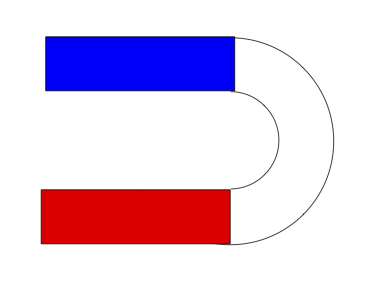
\includegraphics[scale=0.4]{img/horseshoe-magnet}} \\
  %\subcaptionbox{“尾对尾”接在一起的列表}{
    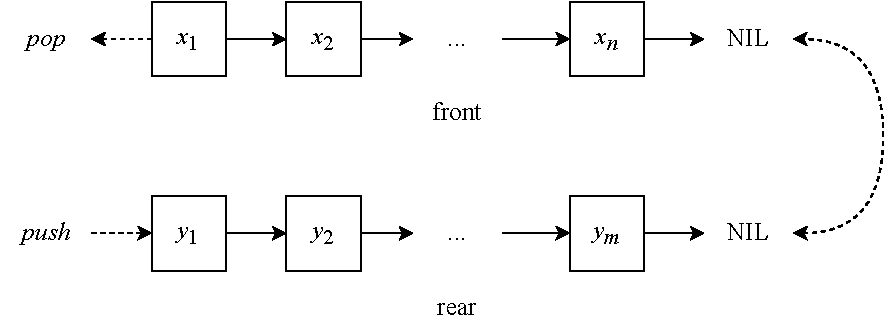
\includegraphics[scale=0.6]{img/paired-listq}
  %}
  \caption{双列表队列}
  \label{fig:horseshoe-magnet}
\end{figure}

\be
\begin{cases}
push\ x\ (f, r) & = (f, x:r) \\
pop\ (x:f, r)   & = (f, r) \\
\end{cases}
\ee

经过一系列出队操作后,$f$可能为空,而$r$中还有元素。为了能继续出队,我们将$r$反转后替换掉$f$:$([\ ], r) \mapsto (reverse\ r, [\ ])$。为此每次出入队后,需要执行一次平衡检查和调整:

\be
\begin{array}{rcl}
\textit{balance}\ [\ ]\ r & = & (\textit{reverse}\ r, [\ ]) \\
\textit{balance}\ f\ r & = & (f, r) \\
\end{array}
\ee

一旦发生$r$的反转,则这次操作的性能下降为线性时间。尽管如此,整体的分摊复杂度是常数时间的。我们重新定义入队和出队为:

\be
\begin{cases}
push\ x\ (f, r) & = \textit{balance}\ f\ (x:r) \\
pop\ (x:f, r)   & = \textit{balance}\ f\ r \\
\end{cases}
\ee

\index{队列!双数组队列}
我们可以用数组给出一个双列表的对称实现。利用表\ref{tab:array-list-comp}的对称性,我们将两个数组“头对头”连接起来形成队列,如图\ref{fig:horseshoe-array}所示。当$R$数组为空时,我们将$F$数组反转替换掉$R$数组。

\begin{table}[htbp]
\centering
\begin{tabular}{l | c | r}
  \hline
  操作 & 数组 & 链表 \\
  \hline
  在头部加入 & $O(n)$ & $O(1)$ \\
  在尾部加入 & $O(1)$ & $O(n)$ \\
  在头部删除 & $O(n)$ & $O(1)$ \\
  在尾部删除 & $O(1)$ & $O(n)$ \\
  \hline
\end{tabular}
\caption{数组和链表各项操作的对比} \label{tab:array-list-comp}
\end{table}

\begin{figure}[htbp]
  \centering
  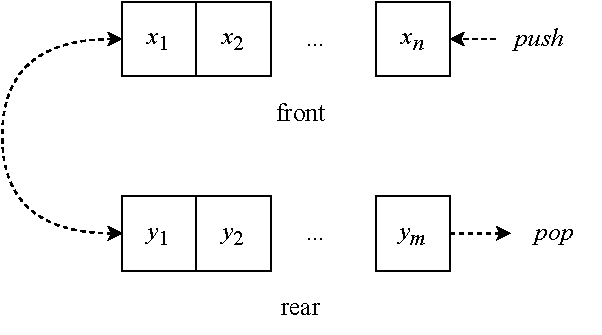
\includegraphics[scale=0.6]{img/paired-arrayq}
  \caption{双数组队列}
  \label{fig:horseshoe-array}
\end{figure}

\begin{Exercise}
\Question{为什么要在push时也要进行平衡检查和调整?}
\Question{证明双列表队列的分摊复杂度为常数时间。}
\Question{实现双数组队列。}
\end{Exercise}

\begin{Answer}
\Question{为什么要在push时也要进行平衡检查和调整?

考虑这样的情况:先$push\ a\ ([\ ], [\ ])$,然后再$pop$。
}
\Question{证明双列表队列的分摊复杂度为常数时间。}
\Question{实现双数组队列。

\begin{algorithmic}[1]
\Function{Push}{$Q, x$}
  \State \textproc{Append}(\Call{Front}{$Q$}, $x$)
\EndFunction
\Statex
\Function{Pop}{$Q$}
  \If{\Call{Rear}{$Q$} $= [\ ]$}
    \State \Call{Rear}{$Q$} $\gets$ \textproc{Reverse}(\Call{Front}{$Q$})
    \State \Call{Front}{$Q$} $\gets [\ ]$
  \EndIf
  \State $n \gets$ \textproc{Length}(\Call{Rear}{$Q$})
  \State $x \gets$ \Call{Rear}{$Q$}[n]
  \State \textproc{Length}(\Call{Rear}{$Q$}) $\gets n - 1$
  \State \Return $x$
\EndFunction
\end{algorithmic}

}
\end{Answer}

\section{平衡队列}
\index{队列!平衡队列}

虽然双列表队列的分摊复杂度为常数时间,但最坏情况下的性能是线性的。例如$f$中有一个元素,此后连续将$n$个元素加入队列,此时执行出队的复杂度为$O(n)$。这一问题的原因是$f$和$r$的长度不平衡。为了改进平衡性,我们加入一条规则,要求$r$的长度不大于$f$的长度,否则就反转列表。

\be
  |r| \leq |f|
\label{eq:balance-invariant}
\ee

每次操作都需要检查长度,但这需要线性时间。为此我们将长度记录下来,并在出入队时更新。这样双列表队列就表示为$(f, n, r, m)$,其中$n = |f|$,$m = |r|$,分别是两个列表的长度。根据平衡规则(\ref{eq:balance-invariant}),我们可以检查$f$的长度来判断队列是否为空:

\be
  Q = \phi \iff n = 0
\ee

我们更新出、入队的定义为:

\be
\begin{cases}
  push\ x\ (f, n, r, m) & = \textit{balance}\ (f, n,  x:r, m + 1) \\
  pop\ (x:f, n, r, m) & = \textit{balance}\ (f, n - 1, r, m) \\
\end{cases}
\ee

其中\textit{balance}定义为:

\be
\textit{balance}\ (f, n, r, m) = \begin{cases}
  m \leq n: & (f, n, r, m) \\
  \text{否则}: & (f \doubleplus reverse\ r, m + n, [\ ], 0)\\
\end{cases}
\ee

\section{实时队列}
\index{队列!实时队列}

在平衡队列的实现中,列表连接、反转的性能仍然是线性时间的。在实时系统中,需要进一步改进。性能瓶颈出现在$f \doubleplus reverse\ r$中。此时$m > n$,违反了平衡规则。由于$m$、$n$都是整数,我们进一步知道:$m = n + 1$。$\doubleplus$的复杂度是$O(n)$,反转操作的复杂度是$O(m)$,总复杂度是$O(n + m)$,和队列中元素个数成正比。我们可以将这一操作分派到各次出、入队中去。首先分析一下尾递归的反转操作:

\be
reverse\ = reverse'\ [\ ]
\ee

这一定义是克里化的,其中:

\be
\begin{array}{rcl}
\textit{reverse}'\ a\ [\ ] & = & a \\
\textit{reverse}'\ a\ (x:xs) & = & \textit{reverse}'\ (x:a)\ xs \\
\end{array}
\ee

可以很容易地将尾递归\cite{wiki-tail-call}\cite{recursion}定义转换为逐步计算。整体过程相当于一系列的状态转换。我们定义一个状态机,包含两种状态:反转状态$S_r$表示正在进行反转(未完成);完成状态$S_f$表示反转已经结束(完成)。接下来我们利用状态机调度调度(slow-down)反转计算:

\be
\begin{array}{rcl}
step\ S_r\ a\ [\ ] & = & (S_f, a) \\
step\ S_r\ a\ (x:xs) & = & (S_r, (x:a), xs) \\
\end{array}
\ee

每一步,我们先检查当前的状态,如果为$S_r$(反转中),但是列表中已没有剩余元素需要反转,就将状态变为完成$S_f$;否则,我们取出列表中的第一个元素$x$,将其链结到$a$的前面。接下来我们不再进行递归,这一步计算到此结束。当前的状态和反转的中间结果被保存下来,供以后再次调用$step$时使用。例如:

\[
\begin{array}{rcl}
step\ S_r\ \text{``hello''}\ [\ ] & = & (S_r, \text{``ello''}, \text{``h''}) \\
step\ S_r\ \text{``ello''}\ \text{``h''} & = & (S_r, \text{``llo''}, \text{``eh''}) \\
... & & \\
step\ S_r\ \text{``o''}\ \text{``lleh''} & = & (S_r, [\ ], \text{``olleh''}) \\
step\ S_r\ [\ ]\ \text{``olleh''} & = & (S_f, \text{``olleh''})
\end{array}
\]

现在我们可以将反转计算逐步分派到出、入队中。但是这仅解决了一半问题。我们需要逐步分解、调度$\doubleplus$。实现逐步连接的难度更大。我们利用逐步反转的结果,并使用一个技巧:为了实现$X \doubleplus Y$,我们可以先将$X$反转为$\overleftarrow{X}$,然后逐一将$\overleftarrow{X}$中的元素取出,放到$Y$的前面。这和$\textit{reverse}'$类似。

\be
  \begin{array}{rcl}
    X \doubleplus Y & = & (reverse\ reverse\ X) \doubleplus Y \\
             & = & (reverse'\ [\ ]\ (reverse\ X)) \doubleplus Y \\
             & = & reverse'\ Y\ (reverse\ X) \\
             & = & reverse'\ Y\ \overleftarrow{X}
  \end{array}
\ee

这一事实表明,我们可以增加另一个状态来控制$step$,在$r$反转后,逐步操作$\overleftarrow{f}$实现连接。三种状态为:反转$S_r$、连接$S_c$、完成$S_f$。整个操作被分解为两个阶段:

\begin{enumerate}
\item 同时反转$f$和$r$,逐步得到$\overleftarrow{f}$和$\overleftarrow{r}$;
\item 逐步从$\overleftarrow{f}$取出元素,链接到$\overleftarrow{r}$前面。
\end{enumerate}

\be
\begin{array}{rcll}
next\ (S_r, f', x:f, r', y:r) & = & (S_r, x:f', f, y:r', r) & \text{同时反转}f, r\\
next\ (S_r, f', [\ ], r', [y]) & = & (S_c, f', y:r') & \text{反转结束、转入连接}\\
next\ (S_c, a, [\ ]) & = & (S_f, a) & \text{连接结束}\\
next\ (S_c, a, x:f') & = & (S_c, x:a, f') & \text{逐步连接}\\
\end{array}
\ee

接下来我们需要将这些递进的步骤分配到每个出、入队操作中以实现实时队列。根据平衡队列的条件,当$m = n + 1$时,我们开始逐步计算$f \doubleplus reverse\ r$。总共需要$n + 1$步来反转$r$,我们同时在这些步骤内完成了对$f$的反转。此后,我们需要再用$n + 1$步来进行连接操作。因此总共花费了$2n + 2$步。最直接的想法是在每一个出、入队中分配一个递进步骤。但这里有一个关键问题:在完成$2n + 2$步操作之前,队列有没有可能由于接下来的一系列出、入队操作再次变得不平衡?

幸运的是,在花费$2n + 2$步完成$f \doubleplus reverse\ r$之前,连续的入队操作不可能再次使队列变得不平衡。一旦开始恢复平衡的处理,经过$2n + 2$步后,我们就得到了一个新的$f$列表$f' = f \doubleplus reverse\ r$。而下一次队列变得不平衡时有:

\be
  \begin{array}{rcl}
  |r'| & = & |f'| + 1 \\
       & = & |f| + |r| + 1 \\
       & = & 2n + 2
  \end{array}
\ee

也就是说,从上次不平衡的时刻算起,即使不断持续入队新元素,以最快的速度再次使得队列不平衡时,$2n + 2$步计算恰好已经完成了。此时新的$f$列表被计算出来。我们可以安全地继续计算$f' \doubleplus reverse\ r'$。多亏了平衡规则,帮助我们保证了这一点。

但不幸的是,在$2n + 2$步计算完成前,出队操作可能随时发生。这会产生一个尴尬的情况:我们需要从$f$列表取出元素,但是新的$f$列表$f' = f \doubleplus reverse\ r$尚未计算好。此时没有一个可用的$f$列表。为了解决这个问题,我们在第一阶段并行计算$reverse\ f$时,另外保存一份$f$的副本。这样即使连续进行$n$次出队操作,我们仍然是安全的。表(\ref{tab:pop-before-n})给出了第一阶段逐步计算(同时反转$f$和$r$)的某个时刻队列的样子\footnote{有人会产生疑问,通常复制一个列表需要花费和列表长度成比例的线性时间。这样整个方案就有问题了。实际上,这一线性时间的列表复制根本不会发生。在函数式环境下,出队或反转并不“修改”$f$列表。为此,我们需要实现某种惰性复制,真正的复制操作并不立即发生,而是在每次反转的递进步骤中一步复制一个元素,见本节练习。}。

\begin{table}[htbp]
\centering
\begin{tabular}{l | l | l}
  保存的$f$副本 & 进行中的计算 & 新的$r$列表 \\
  \hline
  $\{ f_i, f_{i+1}, ..., f_n \}$ & $(S_r, \tilde{f}, ..., \tilde{r}, ...)$ & $ \{ ... \}$ \\
  \hline
  前$i-1$个元素已出队 & $\overleftarrow{f}$和$\overleftarrow{r}$的中间结果 & 包含新入队的元素
\end{tabular}
\caption{前$n$步完成之前的队列中间状态}
\label{tab:pop-before-n}
\end{table}

经过$n$次出队操作,$f$的副本已经用光。我们此时刚刚开始逐步连接的计算阶段。此时如果继续出队会怎样?事实上,由于$f$的副本被用光,变成了$[\ ]$,我们无需再进行连接操作了。这是因为$f \doubleplus \overleftarrow{r} = [\ ] \doubleplus \overleftarrow{r} = \overleftarrow{r}$。事实上,在进行连接操作时,我们只需要将$f$中尚未出队的部分连接起来。因为元素从$f$的头部逐一出队,我们可以使用一个计数器来记录$f$中剩余元素的个数。当开始计算$f \doubleplus reverse\ r$时,计数器为0,每次反转$f$中的一个元素时,就将计数器加一,表示将来我们需要连接这个元素;每次出队操作,就将计数器减一,表示我们将来可以少连接一个元素。显然在连接操作的每步中,我们也需要递减计数器。当且仅当计数器为0的时候,我们无需继续进行连接操作。下面是增加了计数器的状态转换定义:

\be
\begin{array}{rcll}
next\ (S_r, n, f', x:f, r', y:r) & = & (S_r, n + 1, x:f', f, y:r', r) & \text{同时反转}f, r\\
next\ (S_r, n, f', [\ ], r', [y]) & = & (S_c, n, f', y:r') & \text{反转结束、转入连接}\\
next\ (S_c, 0, a, f) & = & (S_f, a) & \text{连接结束}\\
next\ (S_c, n, a, x:f') & = & (S_c, n - 1, x:a, f') & \text{逐步连接}\\
next\ S_0 & = & S_0 & \text{空闲状态} \\
\end{array}
\ee

我们还定义了一个空闲状态$S_0$来简化状态转换的实现。队列的数据结构分为三个部分:$f$列表及其长度$n$、正在计算中的$f \doubleplus reverse\ r$的中间状态、$r$列表及其长度$m$。记为$(f, n, S, r, m)$。空队列记为$([\ ], 0, S_0, [\ ], 0)$。根据平衡规则当$n = 0$时队列为空。我们修改出、入队定义为:

\be
\begin{cases}
  push\ x\ (f, n, S, r, m) & = balance\ f\ n\ S\ (x:r)\ (m + 1) \\
  pop\ (x:f, n, S, r, m) & = balance\ f\ (n - 1)\ (abort\ S)\ r\ m \\
\end{cases}
\ee

其中$abort$在出队时递减计数器,这样将来可以少连接一个元素。我们称其为撤销操作。$balance$检查平衡规则,若不满足则启动$f \doubleplus reverse\ r$逐步恢复平衡;否则执行一步尚未完成的递进计算:

\be
balance\ f\ n\ S\ r\ m = \begin{cases}
  m \leq n: & step\ f\ n\ S\ r\ m \\
  \text{否则}: & step\ f\ (n + m)\ (S_r, 0, [\ ], f, [\ ], r)\ [\ ]\ 0 \\
\end{cases}
\ee

函数$step()$将状态机转换到下一个状态,全部递进计算结束后,状态转换到空闲状态$S_0$。

\be
  step(F, |F|, \mathcal{S}, R, |R|) = \left \{
  \begin{array}
  {r@{\quad:\quad}l}
  Queue(F', |F|, S_0, R, |R|) &  S' = S_f \\
  Queue(F, |F|, \mathcal{S}', R, |R|) & otherwise
  \end{array}
  \right .
\ee

其中,$\mathcal{S}' = next(\mathcal{S})$,是下一个转换到的状态;$F' = F \cup reverse(R)$是递进计算出的新front列表。真正的状态转换函数$next()$的实现如下。和前面的定义不同,我们增加了一个计数器$n$来记录还剩余多少个元素需要连接。

\be
  next(\mathcal{S}) = \left \{
  \begin{array}
  {r@{\quad:\quad}l}
  (S_r, n+1, F', \{ f_1 \} \cup \overleftarrow{F}, R', \{ r_1 \} \cup \overleftarrow{R}) &
      S = S_r \land F \neq \phi \\
  (S_c, n, \overleftarrow{F}, \{ r_1 \} \cup \overleftarrow{R}) &
      S = S_r \land F = \phi \\
  (S_f, A) & S = S_c \land n = 0 \\
  (S_c, n-1, X', \{ x_1 \} \cup A) & S = S_c \land n \neq 0 \\
  \mathcal{S} & otherwise
  \end{array}
\right .
\ee

相应的Haskell例子程序如下:

\lstset{language=Haskell}
\begin{lstlisting}[style=Haskell]
next (Reverse n (x:f) f' (y:r) r') = Reverse (n+1) f (x:f') r (y:r')
next (Reverse n [] f' [y] r') = Concat n f' (y:r')
next (Concat 0 _ acc) = Done acc
next (Concat n (x:f') acc) = Concat (n-1) f' (x:acc)
next s = s
\end{lstlisting}

函数$abort()$用于指示状态机,由于发生了出队操作,可以少连接一个元素。

\be
  abort(\mathcal{S}) = \left \{
  \begin{array}
  {r@{\quad:\quad}l}
  (S_f, A') & S = S_c \land n = 0 \\
  (S_c, n-1, X' A) & S = S_c \land n \neq 0 \\
  (S_r, n-1, F, \overleftarrow{F}, R, \overleftarrow{R}) & S = S_r \\
  \mathcal{S} & otherwise
  \end{array}
\right .
\ee

注意当$n = 0$的时候,我们实际上撤销了上一个链接元素的操作,因此返回$A'$而不是$A$作为结果(作为练习,我们请读者来回答这样做的原因)。

下面的Haskell例子程序实现了abort函数。

\lstset{language=Haskell}
\begin{lstlisting}[style=Haskell]
abort (Concat 0 _ (_:acc)) = Done acc      -- 注意:我们回滚(rollback)了一个元素
abort (Concat n f' acc) = Concat (n-1) f' acc
abort (Reverse n f f' r r') = Reverse (n-1) f f' r r'
abort s = s
\end{lstlisting}

我们已经接近最终的结果了。但是仍有一个隐藏的问题必须解决:如果将一个元素$x$放入一个空队列,结果会是:

\[
  Queue(\phi, 1, (S_c, 0, \phi, \{ x \}), \phi, 0)
\]

若此时立即进行出队操作,就会发生错误!虽然上一次$F \cup reverse(R)$的计算已经结束,但是front列表却为空。这是因为还需要额外一步才能从状态$(S_c, 0, \phi, A)$转换到$(S_f, A)$。因此需要进一步调整函数$step()$中的$\mathcal{S}'$如下:

\be
  \mathcal{S}' = \left \{
  \begin{array}
  {r@{\quad:\quad}l}
  next(next(\mathcal{S})) & F = \phi \\
  next(\mathcal{S}) & otherwise
  \end{array}
\right .
\ee

下面的Haskell例子程序体现了这一修改:

\lstset{language=Haskell}
\begin{lstlisting}[style=Haskell]
step f lenf s r lenr =
    case s' of
      Done f' -> RTQ f' lenf Empty r lenr
      s' -> RTQ f lenf s' r lenr
    where s' = if null f then next $ next s else next s
\end{lstlisting} %$

注意这一算法和Chris Okasaki在\cite{okasaki-book}给出的有所不同。Okasaki的算法每次出队、入队执行两步递进计算,而本章中的算法每次只执行一次。因此计算性能的分布更加均匀。

\begin{Exercise}
\begin{itemize}
\item 在$abort()$函数中,当$n = 0$时,为什么需要回滚一个元素?

\item 考虑实时队列的对称实现。选择一门命令式语言,用双数组实现实时队列。

\item 在脚注中,我们提到,使用就地修改的双数组来实现实时队列时,当开始递进计算反转时,不能一次性复制数组,否则就会将性能降低到线性时间复杂度。请实现一个惰性复制(lazy copy),使得每步反转时我们仅复制一个元素。

\end{itemize}
\end{Exercise}


% ================================================================
%                 Lazy Real-time queue
% ================================================================
\section{惰性实时队列}
\index{队列!惰性实时队列}

实现实时队列的关键在于将耗时的$F \cup reverse(R)$计算分解。惰性求值对于这类问题很有帮助。本节中,我们通过惰性求值来寻找更加简洁的方法。

假设存在一个函数$rotate()$可以逐步计算$F \cup reverse(R)$。也就是说,使用一个累积器$A$,下面的两个函数等价

\be
  rotate(X, Y, A) \equiv X \cup reverse(Y) \cup A
  \label{eq:rot-def}
\ee

其中,我们将$X$初始化为front列表$F$,$Y$初始化为rear列表$R$,$A$初始化为空$\phi$。

开始进行轮转(rotate)的条件和前面一样,即$|F| + 1 = |R|$。在轮转过程中,我们始终保持$|X| + 1 = |Y|$作为一个不变式成立。

下面我们来推导轮转的实现,显然,最简单的情况如下:

\be
  rotate(\phi, \{ y_1 \}, A) = \{ y_1 \} \cup A
\ee

记$X = \{ x_1, x_2, ... \}$、$Y = \{ y_1, y_2, ...\}$;而$X' = \{ x_2, x_3, ...  \}$、$Y' = \{ y_2, y_3, ...\}$是$X$和$Y$除去第一个元素以外的剩余元素。递归情况可以推导如下:

\be
  \begin{array}{rcll}
  rotate( X, Y, A ) & \equiv & X \cup reverse(Y) \cup A & \mbox{根据定义(}\ref{eq:rot-def} \mbox{的定义} \\
  & \equiv & \{ x_1 \} \cup (X' \cup reverse(Y) \cup A) & \cup \mbox{操作的结合性} \\
  & \equiv & \{ x_1 \} \cup (X' \cup reverse(Y') \cup (\{ y_1 \} \cup A)) & \mbox{reverse的性质和}  \cup \mbox{的结合性} \\
  & \equiv & \{ x_1 \} \cup rotate(X', Y', \{ y_1 \} \cup A) & \mbox{根据定义(} \ref{eq:rot-def} \mbox{)}
  \end{array}
\ee

归纳上面的两种情况,可以得到最终的轮转算法。

\be
rotate(X, Y, A) = \left \{
  \begin{array}
  {r@{\quad:\quad}l}
  \{ y_1 \} \cup A & X = \phi \\
  \{ x_1 \} \cup rotate(X', Y', \{ y_1 \} \cup A) & otherwise
  \end{array}
\right .
\ee

如果我们惰性执行$\cup$操作,而不是立即进行链接,也就是说,当出队和入队时才执行$\cup$,就可以将$rotate$计算自然分摊到出、入队中。

根据这一思路,我们修改双列表队列的定义,将front列表变成一个惰性列表,然后将它放入一个流(stream)中\cite{SICP}。当某个出、入队操作,造成队列的平衡被破坏,此时有$|F| + 1 = |R|$,为了恢复平衡,我们开始进行惰性轮转计算。这一惰性计算被作为新的front列表$F'$,而新的rear列表为空$\phi$。我们同时维护一个$F'$的副本作为流。

此后,每当进行出、入队操作,我们就强制流执行一个$\cup$操作。这样流就向前执行一步$ \{ x \} \cup F''$,其中$F'' = tail(F')$。我们丢掉$x$,然后用$F''$替换$F'$作为新的流。

当全部流被计算完毕,就可以开始计算另一个轮转。

为了更好地描述这一思路,我们使用Scheme/Lisp给出例子程序。这样可以明确地控制惰性计算。

\lstset{language=Lisp}
\begin{lstlisting}
(define (cons-stream a b) (cons a (delay b)))

(define stream-car car)

(define (stream-cdr s) (cdr (force s)))
\end{lstlisting}

函数\texttt{cons-stream}从一个元素$x$和列表$L$构造一个惰性列表。它并不对列表$L$求值,求值被推迟到\texttt{stream-cdr}中进行。延迟求值可以通过lambda演算来实现\cite{SICP}。

下面的例子程序给出了惰性双列表队列的定义。

\lstset{language=Lisp}
\begin{lstlisting}
(define (make-queue f r s)
  (list f r s))

(define (front-lst q) (car q))

(define (rear-lst q) (cadr q))

(define (rots q) (caddr q))
\end{lstlisting}

一个队列包含三个部分:一个front列表,一个rear列表和一个代表计算$F \cup reverse(R)$的流。对于空队列,这三个部分全部是null。

\begin{lstlisting}
(define empty (make-queue '() '() '()))
\end{lstlisting}

注意,其中的front列表实际上是一个惰性流,因此需要使用流相关的操作。例如下面的函数通过检查front流来判断队列是否为空。

\begin{lstlisting}
(define (empty? q) (stream-null? (front-lst q)))
\end{lstlisting}

入队函数和上一节所介绍的基本相同。我们将新加入的元素放到rear列表前面,然后检查平衡条件,如果不满足就需要恢复平衡。

\be
push(Q, x) = balance(\mathcal{F}, \{ x \} \cup R, \mathcal{R}_s)
\ee

其中$\mathcal{F}$是表示front列表的惰性流;$\mathcal{R}_s$是表示轮转计算的流。相应的Scheme/Lisp例子程序如下:

\begin{lstlisting}
(define (push q x)
  (balance (front-lst q) (cons x (rear q)) (rots q)))
\end{lstlisting}

出队操作和此前相比有一些不同,由于front列表实际是一个惰性流,我们需要进行强制求值,其余部分保持不变。

\be
pop(Q) = balance(\mathcal{F}', R, \mathcal{R}_s)
\ee

其中$\mathcal{F}'$强制对$\mathcal{F}$进行一次求值,相应的Scheme/Lisp例子程序如下:

\begin{lstlisting}
(define (pop q)
  (balance (stream-cdr (front-lst q)) (rear q) (rots q)))
\end{lstlisting}

为了节省篇幅,我们省略了错误处理(例如对空队列进行出队操作的错误等)。

通过从front流中提取元素可以获得队列的头部元素。

\begin{lstlisting}
(define (front q) (stream-car (front-lst q)))
\end{lstlisting}

平衡函数首先检查代表轮转计算的流,如果已经耗尽,就开始一次新的轮转计算;否则它强制对惰性流进行一次求值,消耗掉其中的一个元素。

\be
balance(Q) = \left \{
  \begin{array}
  {r@{\quad:\quad}l}
  Queue(\mathcal{F}', \phi, \mathcal{F}') & \mathcal{R}_s = \phi \\
  Queue(\mathcal{F}, R, \mathcal{R}_s') & otherwise
  \end{array}
\right .
\ee

这里$\mathcal{F}'$被定义来开始一次新的轮转:

\be
  \mathcal{F}' = rotate(F, R, \phi)
\ee

相应的Scheme/Lisp例子程序如下:

\begin{lstlisting}
(define (balance f r s)
  (if (stream-null? s)
      (let ((newf (rotate f r '())))
    (make-queue newf '() newf))
      (make-queue f r (stream-cdr s))))
\end{lstlisting}

分步递进的轮转函数可以根据我们上面的分析给出实现,如下面的Scheme/Lisp例子代码:

\begin{lstlisting}
(define (rotate xs ys acc)
  (if (stream-null? xs)
      (cons-stream (car ys) acc)
      (cons-stream (stream-car xs)
           (rotate (stream-cdr xs) (cdr ys)
               (cons-stream (car ys) acc)))))
\end{lstlisting}

在Scheme/Lisp中,我们可以明确地控制惰性求值。在默认使用惰性求值的编程环境中,例如Haskell,相应的实现可以非常简洁。

\lstset{language=Haskell}
\begin{lstlisting}[style=Haskell]
data LazyRTQueue a = LQ [a] [a] [a] -- front, rear, f ++ reverse r

instance Queue LazyRTQueue where
    empty = LQ [] [] []

    isEmpty (LQ f _ _) = null f

    -- O(1) time push
    push (LQ f r rot) x = balance f (x:r) rot

    -- O(1) time pop
    pop (LQ (_:f) r rot) = balance f r rot

    front (LQ (x:_) _ _) = x

balance f r [] = let f' = rotate f r [] in LQ f' [] f'
balance f r (_:rot) = LQ f r rot

rotate [] [y] acc = y:acc
rotate (x:xs) (y:ys) acc = x : rotate xs ys (y:acc)
\end{lstlisting}

% ================================================================
%                 Short summary
% ================================================================
\section{小结}

在第一章的开头,我们曾经说过队列并不像想象中的那么简单。我们此前给出了许多数据结构和算法的命令式实现和函数式实现,函数式的方法通常会更加简洁和直观。但是,还存在许多领域,需要更多的研究工作来寻找相应的函数式解法。队列是一个非常重要的题目,它是很多纯函数式数据结构的基础。

Chris Okasaki对纯函数式队列进行了集中的研究,给出了许多有益的讨论\cite{okasaki-book}。通过解决纯函数式队列,我们可以使用类似的方法实现双向队列(dequeue),同时在队列头部和尾部高效地进行操作。再前进一步,还可以实现序列(sequence)数据结构,支持快速地连接(concatenate),并最终实现随机访问(random access)以模拟命令式环境中的数组。我们将在下一章解释这些细节。

虽然我们没有提到优先队列(priority queue),但它可以很容易地用前面章节中给出的堆(heap)来实现。

\begin{Exercise}
\begin{itemize}
\item 使用纯函数的方法,实现双向队列,在头部尾部都支持常数时间$O(1)$的元素添加和删除。
\item 选择一门命令式编程语言,利用数组给出双向队列的对称实现。
\end{itemize}
\end{Exercise}

\section{附录:例子程序}

列表实现的入队、出队:

\begin{lstlisting}[language = Bourbaki]
Queue<K> enQ(Queue<K> q, K x) {
    var p = Node(x)
    p.next = null
    q.tail.next = p
    q.tail = p
    return q
}

K deQ(Queue<K> q) {
    var p = q.head.next   //the next of S
    q.head.next = p.next
    if q.tail == p then q.tail = q.head //empty
    return p.key
}
\end{lstlisting}

循环缓冲区的定义:

\begin{lstlisting}[language = Bourbaki]
data Queue<K> {
    K buf[]
    int head, cnt, size

    Queue(int max) {
        buf = Array<K>(max)
        size = max
        head = cnt = 0
    }
}
\end{lstlisting}

使用循环缓冲区的入队、出队:

\begin{lstlisting}
N offset(N i, N size) = if i < size then i else i - size

void enQ(Queue<K> q, K x) {
    if q.cnt < q.size {
        q.buf[offset(q.head + q.cnt, q.size)] = x;
        q.cnt = q.cnt + 1
    }
}

K head(Queue<K> q) = if q.cnt == 0 then null else q.buf[q.head]

K deQ(Queue<K> q) {
    K x = null
    if q.cnt > 0 {
        x = head(q)
        q.head = offset(q->head + 1, q->size);
        q.cnt = q.cnt -1
    }
    return x
}
\end{lstlisting}

\ifx\wholebook\relax \else
\section{参考答案}
\shipoutAnswer

\begin{thebibliography}{99}

\bibitem{PODC96}
Maged M. Michael and Michael L. Scott. ``Simple, Fast, and Practical Non-Blocking and Blocking Concurrent Queue Algorithms''. \url{http://www.cs.rochester.edu/research/synchronization/pseudocode/queues.html}

\bibitem{SutterDDJ}
Herb Sutter. ``Writing a Generalized Concurrent Queue''. Dr. Dobb's Oct 29, 2008. \url{http://drdobbs.com/cpp/211601363?pgno=1}

\bibitem{CLRS}
Thomas H. Cormen, Charles E. Leiserson, Ronald L. Rivest and Clifford Stein. ``Introduction to Algorithms, Second Edition''. The MIT Press, 2001. ISBN: 0262032937.

\bibitem{okasaki-book}
Chris Okasaki. ``Purely Functional Data Structures''. Cambridge university press, (July 1, 1999), ISBN-13: 978-0521663502

\bibitem{wiki-tail-call}
Wikipedia. ``Tail-call''. \url{https://en.wikipedia.org/wiki/Tail_call}

\bibitem{recursion}
Wikipedia. ``Recursion (computer science)''. \url{https://en.wikipedia.org/wiki/Recursion_(computer_science)#Tail-recursive_functions}

\bibitem{SICP}
Harold Abelson, Gerald Jay Sussman, Julie Sussman. ``Structure and Interpretation of Computer Programs, 2nd Edition''. MIT Press, 1996, ISBN 0-262-51087-1 (中文版:裘宗燕 译《计算机程序的构造和解释》)

\end{thebibliography}

\expandafter\enddocument
\fi
